\documentclass[tikz,border=8pt]{standalone}
% Shared look for every TikZ diagram. Load with \input{../../tools/tikz-style.tex}
\usepackage[T1]{fontenc}
\usepackage{lmodern}
\renewcommand{\sfdefault}{lmr}  % diagrams use the same serif as the text
\usetikzlibrary{arrows.meta, positioning, shapes.geometric, calc, fit, backgrounds}
\definecolor{cblue}{HTML}{4C78A8}
\definecolor{corange}{HTML}{F58518}
\definecolor{cgreen}{HTML}{54A24B}
\definecolor{cred}{HTML}{E45756}
\definecolor{cpurple}{HTML}{B279A2}
\definecolor{cgrey}{HTML}{6B6B6B}
\tikzset{
  every picture/.style={font=\sffamily, line width=1.2pt},
  box/.style={draw=#1, fill=#1!12, rounded corners=4pt, align=center, inner sep=7pt, minimum height=1.1cm},
  box/.default=cgrey,
  arrow/.style={-{Stealth[length=3mm]}, draw=cgrey, line width=1.4pt},
  title/.style={font=\sffamily\bfseries\Large},
  note/.style={font=\sffamily\small, text=cgrey, align=center},
}
\AtBeginDocument{\hyphenpenalty=10000 \exhyphenpenalty=10000}

\begin{document}
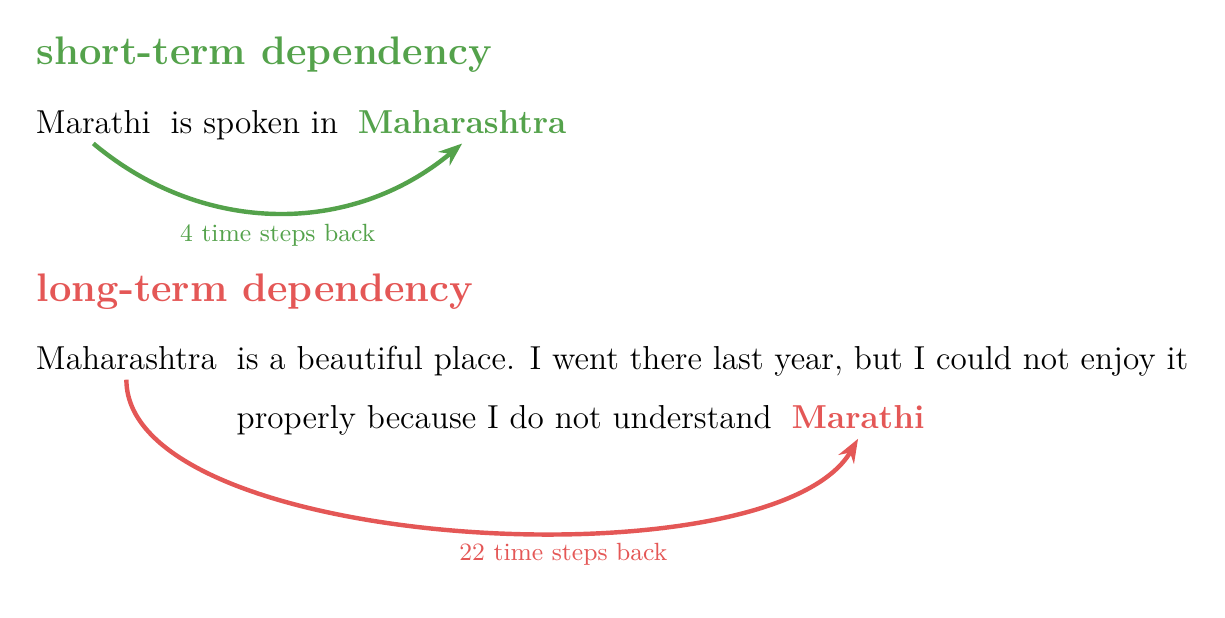
\begin{tikzpicture}[w/.style={font=\sffamily\large, inner sep=3pt, anchor=base west}]
  \node[title, text=cgreen, anchor=west] at (0,1.0) {short-term dependency};
  \node[w] (a1) at (0,0) {Marathi};
  \node[w] (a2) at (a1.base east) {is spoken in};
  \node[w, text=cgreen, font=\sffamily\large\bfseries] (a3) at (a2.base east) {Maharashtra};
  \draw[cgreen, -{Stealth[length=3mm]}, line width=1.6pt] (a1.south) to[out=-40, in=-140] node[below, note, text=cgreen] {4 time steps back} (a3.south);
  \node[title, text=cred, anchor=west] at (0,-2.0) {long-term dependency};
  \node[w] (b1) at (0,-3.0) {Maharashtra};
  \node[w] (b2) at (b1.base east) {is a beautiful place. I went there last year, but I could not enjoy it};
  \node[w] (b3) at ([yshift=-0.75cm]b2.base west) {properly because I do not understand};
  \node[w, text=cred, font=\sffamily\large\bfseries] (b4) at (b3.base east) {Marathi};
  \draw[cred, -{Stealth[length=3mm]}, line width=1.6pt] (b1.south) to[out=-90, in=-120, looseness=0.6] node[below, pos=0.6, note, text=cred] {22 time steps back} (b4.south);
\end{tikzpicture}
\end{document}
